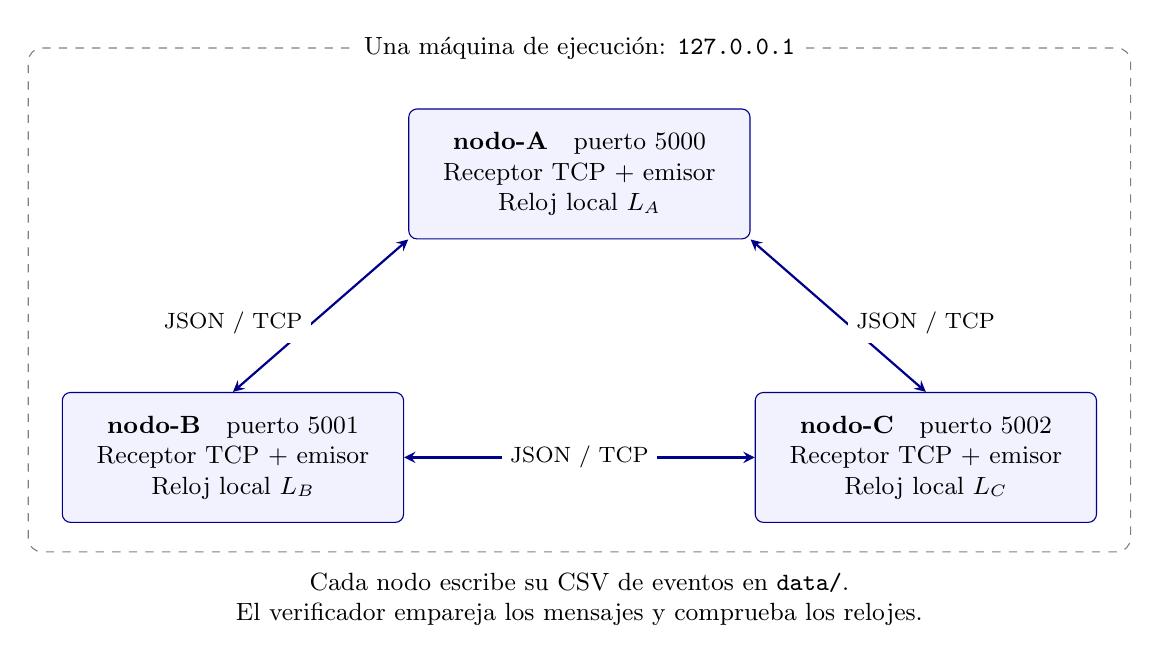
\begin{tikzpicture}[
  servicio/.style={draw=blue!55!black,fill=blue!5,rounded corners=3pt,
    align=center,text width=4.1cm,minimum height=1.65cm,font=\small},
  enlace/.style={<->,>=stealth,thick,draw=blue!55!black},
  etiqueta/.style={fill=white,inner sep=3pt,font=\footnotesize,align=center}
]
\draw[dashed,rounded corners=5pt,gray] (-7,-3.8) rectangle (7,2.6);
\node[font=\small,fill=white] at (0,2.6)
  {Una máquina de ejecución: \texttt{127.0.0.1}};
\node[servicio] (a) at (0,1) {
  \textbf{nodo-A}\quad puerto 5000\\
  Receptor TCP + emisor\\
  Reloj local $L_A$};
\node[servicio] (b) at (-4.4,-2.6) {
  \textbf{nodo-B}\quad puerto 5001\\
  Receptor TCP + emisor\\
  Reloj local $L_B$};
\node[servicio] (c) at (4.4,-2.6) {
  \textbf{nodo-C}\quad puerto 5002\\
  Receptor TCP + emisor\\
  Reloj local $L_C$};
\draw[enlace] (a.south west) -- node[etiqueta,pos=0.55,left]
  {JSON / TCP} (b.north);
\draw[enlace] (a.south east) -- node[etiqueta,pos=0.55,right]
  {JSON / TCP} (c.north);
\draw[enlace] (b.east) -- node[etiqueta] {JSON / TCP} (c.west);
\node[align=center,font=\small] at (0,-4.4) {
  Cada nodo escribe su CSV de eventos en \texttt{data/}.\\
  El verificador empareja los mensajes y comprueba los relojes.};
\end{tikzpicture}
